\documentclass[tikz,border=5pt]{standalone}
\usepackage{amsmath}
\usepackage{pgfplots}
\usepgfplotslibrary{groupplots}
\pgfplotsset{compat=1.18}

\definecolor{corba}{HTML}{365FB3}
\definecolor{punt}{HTML}{B91C1C}
\definecolor{assimptota}{HTML}{6B7280}

\begin{document}
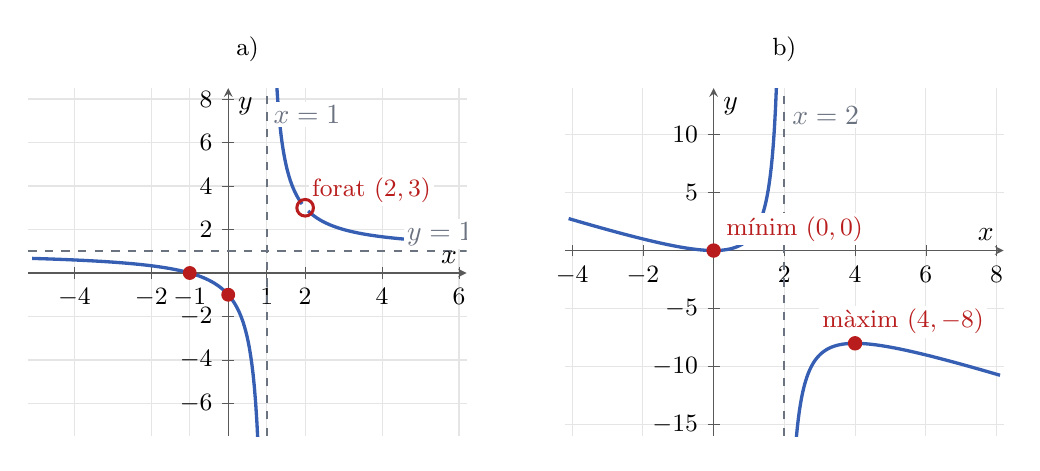
\begin{tikzpicture}
  \begin{groupplot}[
    group style={group size=2 by 1,horizontal sep=1.25cm},
    width=7.15cm,
    height=6cm,
    axis lines=middle,
    xlabel={$x$},
    ylabel={$y$},
    grid=major,
    grid style={black!10},
    axis line style={black!65},
    tick style={black!65},
    tick label style={font=\small},
    title style={font=\small},
    clip=true,
  ]

  \nextgroupplot[
    title={a)},
    xmin=-5.2,
    xmax=6.2,
    ymin=-7.5,
    ymax=8.5,
    xtick={-4,-2,-1,0,1,2,4,6},
    ytick={-6,-4,-2,0,2,4,6,8},
  ]
    \addplot[assimptota, dashed, thick, domain=-5.2:6.2, samples=2] {1};
    \addplot[assimptota, dashed, thick] coordinates {(1,-7.5) (1,8.5)};
    \addplot[corba, very thick, domain=-5.1:0.78, samples=180] {(x+1)/(x-1)};
    \addplot[corba, very thick, domain=1.22:1.92, samples=80] {(x+1)/(x-1)};
    \addplot[corba, very thick, domain=2.08:6.1, samples=150] {(x+1)/(x-1)};
    \addplot[only marks, mark=*, mark size=2.3pt, punt] coordinates {(-1,0) (0,-1)};
    \addplot[
      only marks,
      mark=o,
      mark size=3pt,
      mark options={draw=punt, fill=white, line width=1.1pt}
    ] coordinates {(2,3)};
    \node[anchor=south west, text=assimptota, fill=white, inner sep=1.2pt]
      at (axis cs:4.55,1.08) {$y=1$};
    \node[anchor=south west, text=assimptota, fill=white, inner sep=1.2pt]
      at (axis cs:1.08,6.7) {$x=1$};
    \node[anchor=south west, text=punt, fill=white, inner sep=1.2pt, font=\small]
      at (axis cs:2.08,3.05) {forat $(2,3)$};

  \nextgroupplot[
    title={b)},
    xmin=-4.2,
    xmax=8.2,
    ymin=-16,
    ymax=14,
    xtick={-4,-2,0,2,4,6,8},
    ytick={-15,-10,-5,0,5,10},
  ]
    \addplot[assimptota, dashed, thick] coordinates {(2,-16) (2,14)};
    \addplot[corba, very thick, domain=-4.1:1.78, samples=200] {-x^2/(x-2)};
    \addplot[corba, very thick, domain=2.22:8.1, samples=200] {-x^2/(x-2)};
    \addplot[only marks, mark=*, mark size=2.4pt, punt] coordinates {(0,0) (4,-8)};
    \node[anchor=south west, text=assimptota, fill=white, inner sep=1.2pt]
      at (axis cs:2.12,10.5) {$x=2$};
    \node[anchor=south west, text=punt, fill=white, inner sep=1.2pt, font=\small]
      at (axis cs:0.25,0.45) {mínim $(0,0)$};
    \node[anchor=south east, text=punt, fill=white, inner sep=1.2pt, font=\small]
      at (axis cs:7.75,-7.55) {màxim $(4,-8)$};
  \end{groupplot}
\end{tikzpicture}
\end{document}
